\documentclass[12pt, titlepage]{article}
\usepackage{float}
\usepackage[normalem]{ulem}
\usepackage{color}
\usepackage{graphicx}
\graphicspath{{img/}}
\usepackage{enumitem}
\usepackage{booktabs}
\usepackage{tabularx}
\usepackage{indentfirst}
\usepackage{hyperref}
\usepackage{textgreek}
\hypersetup{
    colorlinks,
    citecolor=black,
    filecolor=black,
    linkcolor=black,
    urlcolor=blue
}
\usepackage[round]{natbib}

\title{SE 3XA3: Software Requirements Specification}

\author{Group 3 - Hextron
		\\ Jason Li lij107
		\\ Scott Williams willis12
		\\ Yousaf Shaheen shaheeny
}

\date{December 6, 2017}



\begin{document}

\maketitle

\pagenumbering{roman}
\tableofcontents
\listoftables
\listoffigures


\begin{table}[]
\caption{\bf Revision History}
\begin{tabularx}{\textwidth}{p{3cm}p{2cm}X}
\toprule {\bf Date} & {\bf Version} & {\bf Notes}\\ 
\midrule
October 6, 2017 & 1.0 & Revision 0 \\ \hline
December 6, 2017 & 1.1 & \begin{itemize}[leftmargin=0cm,itemindent=.5cm,labelwidth=\itemindent,labelsep=0cm,align=left,itemsep = 0mm,nosep]

  \item Changed the description for Functional Requirement 3 to be more detailed.
  \item Added Functional Requirement 7 outlining the rainbow trapezoids.
  \item Added Functional Requirement 8 outlining the black trapezoids.
  \item Removed Health and Safety Requirement 1 which outlined the epilepsy warning (not needed).
  \item Added Health and Safety Requirement outlining a warning that will be given after 30 minutes of continuous play.
  \item Made some minor terminology description changes.
  \item Added Functional Requirement 9 outlining the tips and instructions. 
  \item Added Functional Requirement 10 outlining background music and sound effects.
  \item Added Functional Requirement 11 outlining the leaderboard.
  \item Added Functional Requirement 12 outlining block  elimination edge cases.
  \item Modified some non-functional requirements to provide a better description.
  \item Extended section 4.7 Costs to discuss testing.
  \item Added to User Documentation and Training to facilitate new additions to the game.
  \item Added use case diagram.

  
  
  
\end{itemize} \\
\bottomrule
\end{tabularx}
\end{table}

\vspace*{\fill}
\newpage

\pagenumbering{arabic}

\section{Project Drivers}
This section outlines the basics of the project including purpose, stakeholders, constraints, etc.

\subsection{The Purpose of the Project}
The purpose of this project is to recreate the puzzle game Hextris. We will also be adding new content in order to make the product distinct from another recreation that was done in a past year. Additional content such as powerups and additional shape modes will improve upon the base game. We are recreating the project also to improve our skills and experience in terms of learning the software development lifecycle.

\subsection{The Stakeholders}
There are many stakeholders in this project who are in different positions. Stakeholders are people who will interact with and are affected by the final project. This includes many different people of different positions. Stakeholders also include the people involved in the development of the project. In addition, the developers, professor and teaching assistants are also stakeholders in this project as they provide guidance and assistance in the development process. Other stakeholders include our friends and colleagues who are taking the same course and some of which will be offering feedback.


\subsubsection{The Client}
The client stakeholder involved in this project is the Professor, Dr. Ashgar Bokhari. The client stakeholder is the person who seeks out a team of developers in order to solve a particular problem. Although Dr. Ashgar Bokhari did not present a problem necessarily, he came to us with a task to complete. Dr. Ashgar Bokhari will assess the final product once the deadline comes and will appoint a grade point to quantify the quality of the final product. This assessment will affect our final grade in the course. Overall, Dr. Ashgar Bokhari is the main stakeholder involved in this project.

\subsubsection{The Customers (Users)}
The secondary stakeholders in this project include the students taking the 3XA3 course. The customer, or users, stakeholders are the people who will be utilizing the final product made by the team of developers. The users include mainly the students in the course, but also involve the friends and family of the stakeholders. The users will provide feedback and critique on the product, which will be useful if the team decides to further develop and improve the final product. The customer/users stakeholders in a development project are very important if the development team wants to improve their product or make any changes needed. Secondary stakeholders in a project can often be more important for a project, especially for future development.

\subsubsection{Other Stakeholders}
The developers are also a stakeholder in this project, this includes the 3 group members in group 3. We were tasked by Dr. Bokhari to recreate and improve upon an existing project in order to improve our software development and teamwork skills. We are charged with developing Hextris in the Unity platform as well as any other aspects in regards to the life cycle of the project. We will ensure that the game runs as intended given our own set requirements. Our grade for the project will be determined by the primary stakeholder (client). Collectively, the developers assigned to Hextris are secondary stakeholders.

\subsection{Mandated Constraints}
\begin{enumerate}[label=C\arabic*]
\item \textbf{Fit Criterion:} The product shall operate in a Windows environment. {\color{blue}The program will be able to be run from an executable for simplicity.} \\
\textbf{Rationale:} The client will use Windows and will not change their operating system in order to run the Unity project. The windows environment is a common and easily accessible platform.\\
\textbf{Fit Criterion:} The project shall be run on another Windows machine outside each of the laptops that group members use for implementing Hextris. 

\newpage

\item \textbf{Description:} The development group cannot plagiarise upon the discretion of the professor stakeholder. \\
\textbf{Rationale:} A big part of this project is that we have to recreate the project from scratch. \\
\textbf{Fit Criterion:} The professors and teaching assistants who are assigned with guidance of the group have the tools to ensure that no code is being directly copied between projects. 
\end{enumerate}



\subsection{Naming Conventions and Terminology}
\noindent \textbf{Windows:} Refers to the Microsoft created Operating system \sout{not a physical light opening in a house}.\\
\textbf{Unity:} Refers to the Unity game engine. \sout{not a sense of joined or being whole}.\\
\textbf{C\#:} Is a programming language which Unity predominantly use.; \sout{doesn't refer to the musical note}.\\
\textbf{TA:} Teaching Assistant\\
\textbf{Actor:} Stakeholders of the system that are acknowledged in the requirements document. This does not refer to an actor involved in theatrical productions on either the stage or in film.\\
\subsection{Relevant Facts and Assumptions}

The user is able to manipulate and use a keyboard to access the left and right arrow keys in order to play the game. The user will also have access to a computer which can run the game program on a Windows Operating System. We are also assuming that the user is able to read and understand english. The game will not be available online as the project is intended for educational purposes and not for monetization. The game will not keep scores as an online leaderboard, but will instead be locally saved to keep track of personal scores. The game will not offer any sort of personal customization and will be uniform for all users.

\newpage
\section{Functional Requirements}
This section outlines the functional requirements for the project.

\subsection{The Scope of the Work and the Product}
The boundary between the different actors of the system must be identified. The boundary should encapsulate the internal implementation, as well as the external view by the users. In this situation, the Hextris development team has access to both views. What this entails is that the team is tasked with creating the product by fulfilling all functional and non-functional requirements within the confinements of the constraints. There are several use cases that the group is related to, which includes the development of system timers, color schemes, and base functionality of the puzzle game. The users are directly involved in starting the game through the menu screen, pausing the game, as well as different inputted keys to move a center hexagon. The teaching assistants and professor will also have similar use cases, with the exception of them distinctly assessing the project in different phases of the development cycle. The combination of all these use cases captures the product scope. 

%use case diag
\begin{figure}[H]
\centering
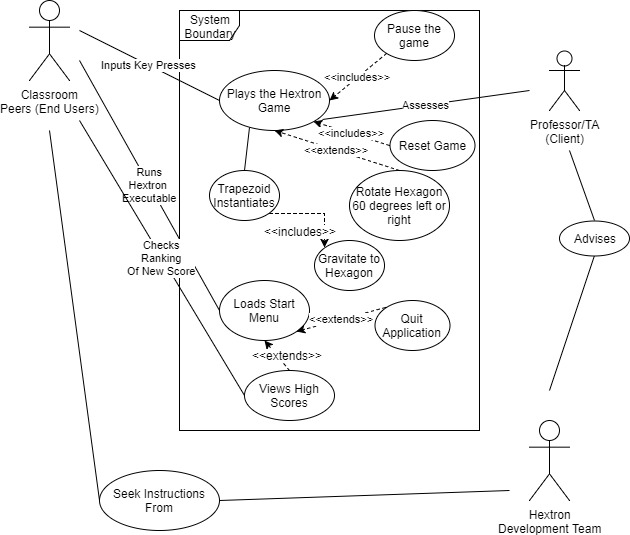
\includegraphics[width=12cm]{HextronUseCase}
\caption{Use Case Diagram}
\end{figure}

\subsubsection{The Context of the Work}
The context of the program indicates that there are various subject domains that need to be fully understood by each member of the team. Firstly, the Unity domain must be understood as the modelling of different game scenes takes place within the game engine. Additionally, the Windows domain must be understood, since the executable project file must be run within the operating system environment.


\subsection{Functional Requirements}
\begin{enumerate}[label=F\arabic*]
\item \textbf{Description:} The program shall generate randomly selected colored blocks of either red, blue, yellow, and green after the start of the game.\\
\textbf{Rationale:} This exists because the group is tasked with recreating the Hextris game. This is in addition to adding our own features to distinguish what we create versus what has already been done before. The different colored blocks are an integral part of the software system, and is an absolute necessity for the game to work like it is meant to. \\
\textbf{Fit Criterion:} A system timer will find the time between when the first block is generated and when the second block is generated. If that time is three seconds, then the requirement has been fulfilled. 

\item \textbf{Description:} The Hextris program colored blocks must be able to approach the center hexagon within a time rate of \textdelta \space at the start of the Hextris game.\\
\textbf{Rationale:} This is mandatory since the blocks must approach the center hexagon to either land on the polygon itself or to land on top of another block. This is how the game progresses and functions. \\
\textbf{Fit Criterion:} A system timer in testing will find the time from when the first block is generated and when it collides with the center hexagon object. If that time is \textdelta, then the requirement is fulfilled. 

\item \textbf{Description:} The game shall increase the rate in which blocks are generated \sout{and the blocks movement speed towards the center polygon by \textalpha \space every minute for a maximum of four minutes.} {\color{blue}by \textalpha \space every 10 seconds until maximum spawn rate has been reached.}\\
\textbf{Rationale:} This is to create a pacing for the game such that there is a smooth transition to a tougher difficulty. Since this is a puzzle game, it is common nature for this to be done as it is important for the user to think at a faster rate as they keep playing. It also provides a lasting appeal to the user to keep coming back to playing, since they will want to improve their reflexive thinking skills.\\
\textbf{Fit Criterion:} The game will have a velocity tracker for the blocks between two different times for colliding objects like the blocks. This velocity will be recorded at differences of a minute between times. 

\item \textbf{Description:} The game shall support up to eight different colored blocks on each hexagon side, with an additional ninth block resulting in a game over screen. \\
\textbf{Rationale:} The original Github project for Hextris had a working demo that could be found on the internet. This version had it so that the game over screen was reached once nine blocks were stacked on top of each other on a hexagon side. Since our job is to recreate Hextris, this is what is required of the development team. \\
\textbf{Fit Criterion:} Black box testing will be used by one of the project members to create a condition in which blocks are simply stacked on top of each other for a game over screen. 

\item \textbf{Description:} The Hextris project must rotate the center hexagon in the direction of a left or right arrow key input by \textepsilon. \\
\textbf{Rationale:} In the context of this game, the hexagon must be able to rotate or else there will be no sense of control for the user. If there is no control, then the game ceases to be interactive and is not a puzzle video game. \\
\textbf{Fit Criterion:} White box testing will ensure that a point of the hexagon will rotate by \textepsilon \space in the direction of a key press through a conditional statement at the start of the game. 

\item \textbf{Description:} The game shall have a key binding such that the game can be paused until the user decides to continue the game by pressing that same key.\\
\textbf{Rationale:} Most video games have a pause button so the user can take an indefinite amount of time to do something else and come back to where they left off. It makes sense for the Hextris recreation to incorporate the same feature. \\
\textbf{Fit Criterion:} White box testing will be used to ensure that no code is running once the user clicks on the pause key binding. 

{\color{blue} %begin blue coloring
\item \textbf{Description:} The system shall generate rainbow colored trapezoids that, upon landing, destroy all objects surrounding it\\
\textbf{Rationale:} Our team members were tasked with adding new features to the gameplay, and one of which we decided was rainbow colored blocks that work will all sorts of blocks.\\
\textbf{Fit Criterion:} There shall be a dynamic, automated test that generates four blocks around a common position. The rainbow colored block will spawn and after a period 5 seconds, the test will check if all objects are destroyed on the screen.

\item \textbf{Description:} The system shall generate black trapezoids that refuse to work with other types of trapezoids (including black ones), except for the rainbow colored one.\\
\textbf{Rationale:} We feel as this addition will add to the difficulty and strategy of the game because the user should try and leave open space for the black trapezoid upon landing. This is because rainbow trapezoids will spawn in the future and be able to destroy it and free up space on the grid.\\
\textbf{Fit Criterion:}  Black box testing will ensure this feature is successfully implemented.


\item \textbf{Description:} The game will have tips and instructions to play the game as well as to help players improve their score. \\
\textbf{Rationale:} While intuitive, the game still has elements that could be confusing for players completely new. Basic instructions should be given as to guide new players. Additionally tips  are a common part of most games assisting in progressing players once they have reached a roadblock. \\
\textbf{Fit Criterion:} User feedback testing will be used to ensure that the instructions and tips are present as well as providing effective assistance to new players .

\item \textbf{Description:} Background music as well as sound effects will be added to block destructing and idling.\\
\textbf{Rationale:} Many games make use of music and other sound based stimulus to improve the overall feel of the game as well as to indicate certain events that have occurred. The music will add to the enjoyment of the game overall.\\
\textbf{Fit Criterion:}  User feedback testing will ensure that the music is working as well as being a good fit to the game and adding to the experience.

\item \textbf{Description:} A local highscore will be added to record the player's top 5 scores keeping track of them locally within the game.\\
\textbf{Rationale:} To encourage players to improve their performance in the game their top scores need to be recorded. It will also increase replay ability as players try to improve their scores.\\
\textbf{Fit Criterion:} White box testing will be used to ensure that the recorded score are working as intended and will save the correct information.

\item \textbf{Description:} Block elimination will need to account for match any number of blocks of the same colour assuming that there are more than 3 of the same colour is provided. The elimination will also need to account for blocks underneath other blocks are eliminated and fall towards the center.\\
\textbf{Rationale:} There will be instances where falling blocks will connect more than 3 blocks of the same colour at once, these niche cases also need to be accounted for as if not eliminated they will cause the game to fail in leaving combinations of blocks that should be eliminated stay on board.\\
\textbf{Fit Criterion:} Dynamic unit testing will be used for specific edge case generation as multiple different combinations can be formed and need to be covered. The automated testing will ensure that no combination of blocks can cause the program to fail.
}%End blue coloring

\end{enumerate}


\section{Non-functional Requirements}
This section outlines the non-functional requirements for the project.



\subsection{Look and Feel Requirements}
\begin{enumerate}[label=LF\arabic*]
\item \textbf{Description:} The visual aspects of the final product is intended to be simple, yet appealing. The GUI and other visual aspects of this project is meant to be developed using sprites from the Unity game engine. The control system also has to be of high quality.\\
\textbf{Rationale:} The feel of the product has to be responsive. In a game such as this, the control system has to be very responsive in order to achieve quality gameplay.\\
\textbf{Fit Criterion:} To achieve this, we will make sure to minimize input lag and optimize collision detection. {\color{blue}Survey testing will need to be done with feedback to be provided by the testers on the visual impact of the game as well as the GUI overall.}

\end{enumerate}

\subsection{Usability and Humanity Requirements}
\begin{enumerate}[label=UH\arabic*]
  \item \textbf{Description:} The final project will be using a Windows PC, and as such it will be controlled using a mouse and keyboard. This means that the control system has to make sense and is relatively simple to understand.\\
\textbf{Rationale:} The user should be able to grasp the control system very easily. In addition, there has to be a limited number of buttons used for controls, since if too many buttons are used, it becomes difficult to remember the functionality of each individual button.\\
\textbf{Fit Criterion:} To achieve this, we will make sure to have a limited number of actions the user can perform. This is instead focusing more on strategy. Thus decreasing the number of button required.

\end{enumerate}

\subsection{Performance Requirements}
\begin{enumerate}[label=P\arabic*]
\item \textbf{Description:} Hextris is an arcade game that is based on strategy, and more importantly reaction time. As such, the software must perform at \textgamma \space to not hinder the user due to any performance drops.\\
\textbf{Rationale:} If there are many performance drops causing delays in the updating of the GUI, it could possibly produce a situation that is unjust for the user. For this reason, the program has to perform well enough to not hinder and negatively affect a user's reaction time.\\
\textbf{Fit Criterion:} To achieve this, we  will make use of efficient algorithms and use minimalistic graphics in order to reduce system requirements. The checking will be through certain Windows tools that check performance of games currently running. 

\end{enumerate}

\subsection{Operational and Environmental Requirements}
\begin{enumerate}[label=OR\arabic*]
\item \textbf{Description:} This program must be compatible with Windows and has to run on a PC.\\
\textbf{Rationale:} An arcade game such as this is most easily played with a mouse and keyboard on a PC.\\
\textbf{Fit Criteria:} This project will be created using Unity game engine and thus will be able to run on a PC.

\end{enumerate}


\subsection{Maintainability and Support Requirements}
\begin{enumerate}[label=M\arabic*]
\item \textbf{Description:} The project must be update-able.\\
\textbf{Rationale:} If a game breaking bug is discovered, the {\color{blue}programmer charged with maintaining the game} \sout{client} needs to be able to provide an update or patch to fix the bug. \\
\textbf{Fit Criterion:} The client or developer can release a new and updated application for people to download again. This is feasible since the application won't be a big file and would be quick to install.

\end{enumerate}



\subsection{Security Requirements}
\begin{enumerate}[label=S\arabic*]
\item \textbf{Description:} There are minimal security requirements for an application such as this. The program will only need to write a small amount of data onto the computer.\\
\textbf{Rationale:} Many applications steal data from a computer through malicious software hidden behind games or other appealing applications.\\
\textbf{Fit Criterion:} This can be achieved easily. The product does not need to read data from the computer other than the high scores data that the application will write onto the computer.

\end{enumerate}



\subsection{Cultural Requirements}
\begin{enumerate}[label=C\arabic*]
\item \textbf{Description:} The Hextris project must be culturally inoffensive towards all end users of our product. \\
\textbf{Rationale:}  Certain video games are controversial due to their imagery, such as how Wolfenstein is synonymous with Nazi imagery. Puzzle games are rarely or never offensive, since the point of them is to encourage critical thinking. \\
\textbf{Fit Criterion:} Other than instructions and warnings regarding health and safety, the program will not contain any text at all. This measurement ensures that no one will be offended by the design of the game. {\color{blue}Additionally with feedback testing we will take into account if any part of the program present any offensive wording/imagery.}

\end{enumerate}
\subsection{Legal Requirements}
\begin{enumerate}[label=L\arabic*]
\item \textbf{Description:} The project must include the GPL v3 license, such that derivative works contain the same user rights that our own project has. \\
\textbf{Rationale:} The original version of Hextris on Github contains a GPL v3 license which is copyleft. This mentions that free use is applicable so long as the same rights are applied to future successors of the project. \\
\textbf{Fit Criterion:} The Teaching Assistant stakeholders who mark our project ensures that the Git repository is organized every milestone, so it will be promptly checked by different stakeholders.

\end{enumerate}

\subsection{Health and Safety Requirements}
\begin{enumerate}[label=HS\arabic*]

\item \sout{\textbf{Description:} The Hextris project shall give warnings upon starting of their first game within the play session that if the user has a history of epilepsy or any seizure activity, they are advised to consult a doctor before playing the game. \\
\textbf{Rationale:} Certain video games, particularly 16-bit games, have the potential to cause seizures. This is possible through different patterns that are subjected to the view of the end users, including flashing colors and other visual cues. }


\item \textbf{Description:} \sout{The system shall give a warning after 30 minutes of playtime to the user for them to consider taking a break from playing Hextris.} {\color{blue}The system shall give a warning to the user for them to consider taking a break from playing Hextris after long play sessions.}\\
\textbf{Rationale:} Due to the nature of repetitive motion, video games are responsible for causing certain medical conditions that put stress on parts of the hand. This includes carpal tunnel syndrome, tendinitis, among other implications. There is also the scenario of video games causing eye strain after excessive playtime, since continuously looking at a pixelated screen results in dryness of the eyes.


\end{enumerate}




\section{Project Issues}
This section discusses potential issues with the project.

\subsection{Open Issues}
One open issue is the balance of the game regarding addition of powerups and new content. When adding new features it will disrupt the difficulty of the game and if the game becomes too skewed towards easy or hard difficulty, we will need to alter the additions to make sure the game stays relatively the same in concept. We may need to implement or remove features based on the difficulty after the changes. 

\subsection{Off-the-Shelf Solutions}
One potential solutions would be the actual project of Hextris not assisting in our additional content. That being said, it will help in terms of the actual base game. However, seeing as reading the open sourced code conflicts against the main idea of the project (building upon a project through the entire software development cycle), this solution should be avoided if possible. Other possible solutions come from the Unity engine, as it provides pre built scripts for necessary objects such as colliders and physics. These are useful and is the primary reason we chose the Unity engine.

\subsection{New Problems}
One potential user problem would be the negative reaction from the new alterations to the game. With new features and powerups the game will change and users may not appreciate the new elements to the game. This feedback will be taken into consideration based on the testers that we will have once the new features have been implemented. We will consider their feedback as well as our own personal feedback and adjust power ups accordingly. 

\subsection{Tasks}
The tasks needed to complete the game will be broken down into 2 sections, development of the base game, and additional features. 

\begin{enumerate}
\item 
\begin{itemize}
\item Implementation of the base collision scripts and block generation
\item Importing visuals for the block, base and player
\item Linking the scripts to the graphics
\item Writing player control, score and block elimination scripts
\end{itemize}

\item
\begin{itemize}
\item Writing script and adding visuals for new type of blocks.
\item Adding pause feature and adding safety messages to menus
\item Reorganizing visuals and code to allow different shapes to be played
\end{itemize}
\end{enumerate}

\subsection{Migration to the New Product}
First conversion to technology is from unity to visual studio from working with the visuals to writing game scripts. Since Unity has built in support and link to visual studios, data transfer and link will be a factor of click and drop. Another translation is when testing comes around, as we will be needing to transition to Visual Studio's built in Unity test tools.  Again, the systems are compatible so transitions to this should be very straightforward.


\subsection{Risks}
\begin{itemize}
\item Game imbalance
\item Overestimated work speed
\item Unfamiliar environment
\item Undesired upgrades
\item Low productivity
\end{itemize}

\indent The biggest risk that we have are the overestimated work speed and unfamiliar environment. The shear amount of work in combination with having to learn many new functions will significantly increase the amount of time spent on the project and progress. 


\subsection{Costs}
In terms of monetary costs, the estimation for our project should be close to 0. This is because our environment and used resources are free, for the most part. In terms of time, the actual base game should take around 50 man hours and additions ranging from anywhere between 10 and another 30 hours. As the additions mostly build off the base game so the majority will have to be spent on the base game. {\color{blue}After the implementation there will be approximately 20 man hours dedicated to testing of the game to ensure playability as well confirming that the game fit the set requirements to a acceptable amount.}

\subsection{User Documentation and Training}
In terms of documentation for player use, the game will have basic control instructions to inform players how to earn points and control the shape. The documentation will be built into the beginning of the game. {\color{blue}The game will have an option to open the instructions on how the game is intended to be played.
}\\

The plans, requirements and any other document related to the life cycle of the game will need to be submitted to the client (Dr. Bokhari and Jean) so that we can receive feedback as well as a grade. We as the developers need to maintain the documents, to make sure that they are up to date.


\subsection{Waiting Room}
There are no current plans for future releases of our version, after we are finished with the submission. In consequence, no new requirements will be considered for new releases after the final demonstration at semesters end. 

\subsection{Ideas for Solutions} 
Solution for new functions in Unity: there are multiple tutorials online by Unity or by other users, some of which have solutions to similar shapes and ideas, we can gather some ideas from those videos if we become stumped by issues related to various Unity functions. 



\newpage
\section{Appendix}

\subsection{Symbolic Parameters}
\noindent \textepsilon \space is a 60 degree angle. 
\newline
\textdelta  \space represents 3 seconds.
\newline
\textalpha \space  represents 25\%.
\newline
\textgamma \space represents 30 frames per second.



\subsection{Modification to Original Document Template}
\begin{itemize}
\item Section 1.2.2 The Customers changed to The Customers (Users)
\item removed subsubsection{Work Partitioning}
\item subsubsection{Individual Product Use Cases}
\item removed List Of Figures
\end{itemize}






\end{document}
